\chapter{Efficiency and Time Resolution Fit Parameters} % (fold)
\label{cha:efficiency_and_time_resolution_fit_parameters}

\section{Efficiency Vs $E_{gain}$} % (fold)
\label{sec:efficiency_vs_egain}
\begin{figure}[!htbp]
\centering
% 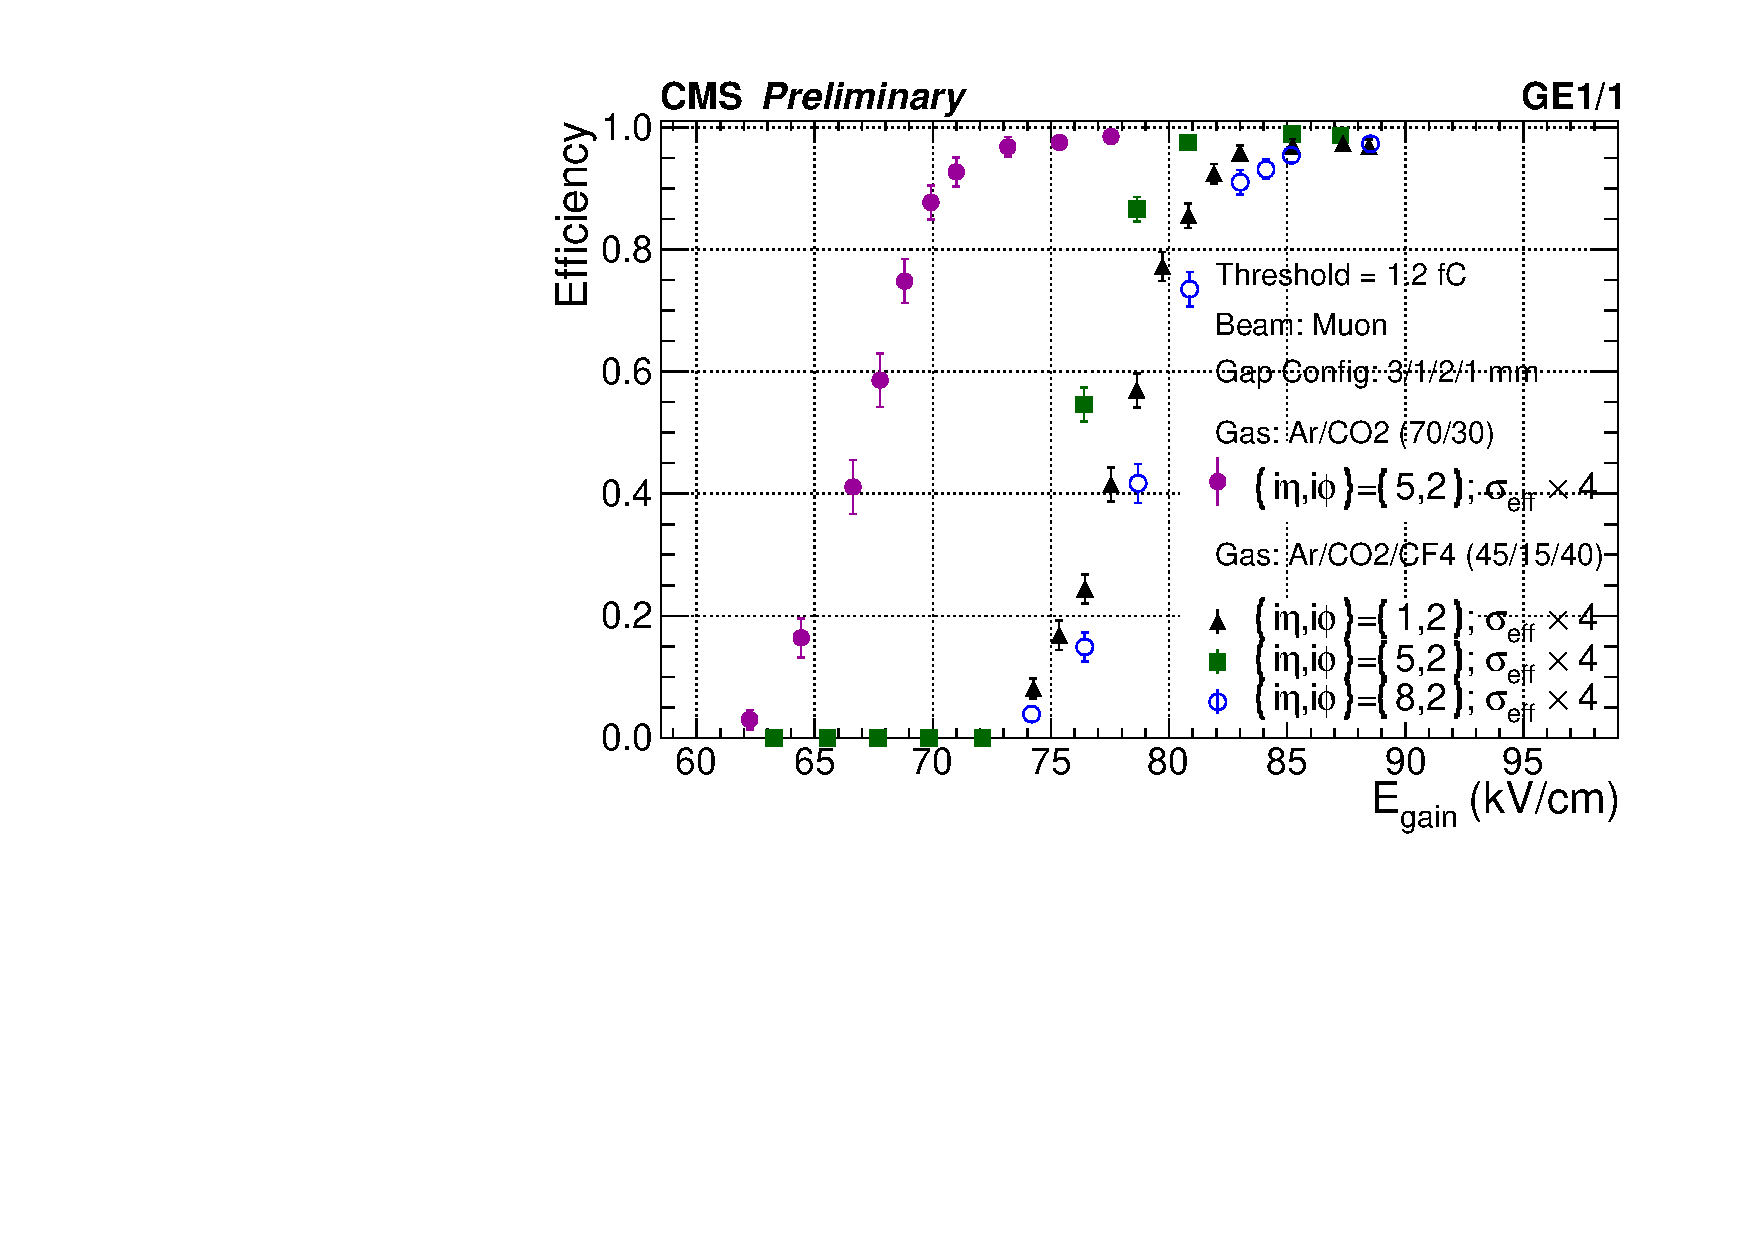
\includegraphics[width=3.5in]{figures/GEM/EfficiencyPlot_wrt_EGain_wError4times_2gas.pdf}
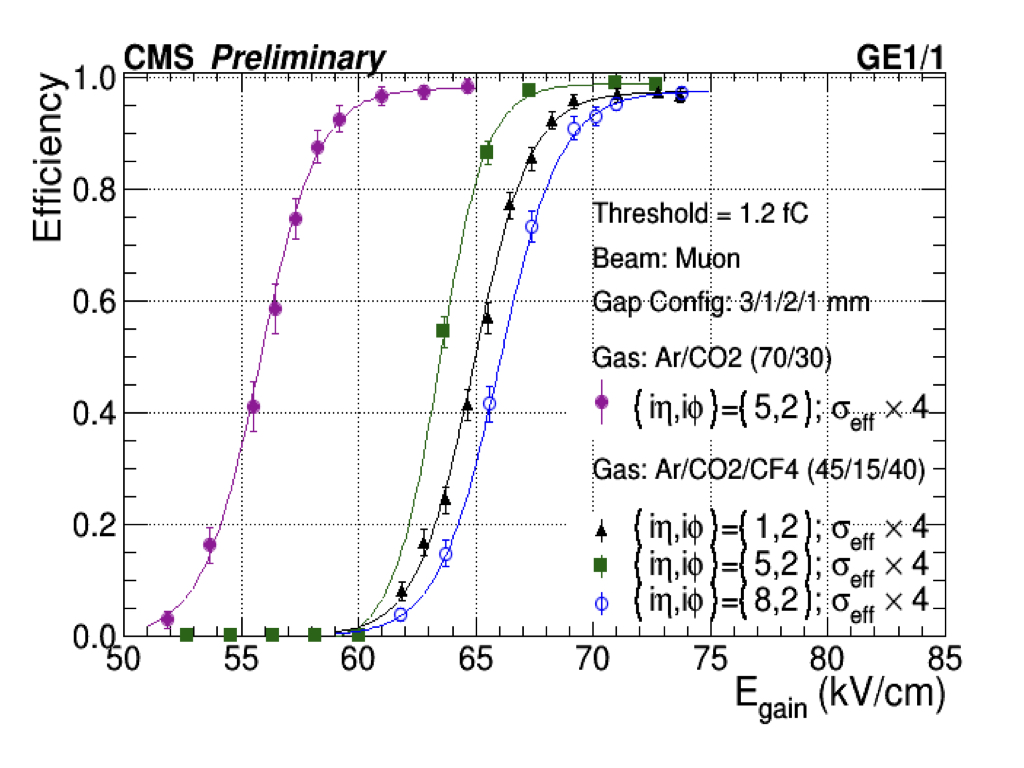
\includegraphics[width=0.75\textwidth]{figures/GEM/Efficiency_EGain.jpeg}
\caption{Efficiency w.r.t. $E_{gain}$ for two different gases and three different $(i\eta,i\phi)$ sectors.}
\label{Efficiency1}
\end{figure}
Here, the efficiency is fitted with function:
\begin{equation}\label{EfffitEq}
    Efficiency = \frac{Eff_{max}}{1+e^{s(HV-HV_{50\%})}}
\end{equation}
Where, $Eff_{max}$ is the maximum obtained efficiency, $HV_{50\%}$ is the applied HV (or current or $E_{gain}$) when corresponding efficiency becomes 50\% and $s$ is just a scale factor.

\subsection{Fit Parameters} % (fold)
\label{sub:fit_parameters}
Lets define four different function, based on equation~\ref{EfffitEq}, F1 for $(i\eta,i\phi)$ sector (5,2) with gas $Ar/CO_2/CF_4$, F2 for $(i\eta,i\phi)$ sector (1,2) with gas $Ar/CO_2/CF_4$, F3 for $(i\eta,i\phi)$ sector (8,2) with gas $Ar/CO_2/CF_4$ and F4 for $(i\eta,i\phi)$ sector (5,2) with gas $Ar/CO_2$.
% subsection fit_parameters (end)

After fit F1 is given as
\begin{equation}
	F1 = [0] + \frac{0.989}{[1]+exp(-[2]\times(x-63.43))}
\end{equation}
where,
% $[0] = -1.44526e-02 \pm 4.28771e-02$, \\$[1] = 9.84833e-01 \pm 4.19715e-02$ and \\$[2] = 9.97591e-01 \pm 8.53940e-02$
\begin{align*}
[0] &= -1.44526e-02 \pm 4.28771e-02,\\
[1] &= 9.84833e-01 \pm 4.19715e-02,~and \\
[2] &= 9.97591e-01 \pm 8.53940e-02
\end{align*}

After fit F2 is given as
\begin{equation}
	F2 = \frac{0.968}{[0]+exp(-[1]\times(x-64.9))}
\end{equation}
where,
\begin{align*}
[0] &= 9.92180e-01 \pm 5.56034e-03,\\
[1] &= 8.25180e-01 \pm 3.62098e-02
\end{align*} 

After fit F3 is given as
\begin{equation}
	F3 = \frac{0.973}{[0]+exp(-[1]\times(x-66))}
\end{equation}
where,
\begin{align*}
[0] &= 9.96407e-01 \pm 9.00503e-03, \\
[1] &= 7.67029e-01 \pm 4.59276e-02
\end{align*}


After fit F4 is given as
\begin{equation}
	F4 = \frac{0.985}{[0]+exp(-[1]\times(x-55.8))}
\end{equation}
where,
\begin{align*}
[0] &= 1.00305e+00 \pm 7.91473e-03,\\
[1] &= 8.15287e-01 \pm 5.46309e-02
\end{align*}



% section efficiency_vs_ (end)


\section{Efficiency Vs current} % (fold)
\label{sec:efficiency_vs_current}
\begin{figure}[!htbp]
\centering
% 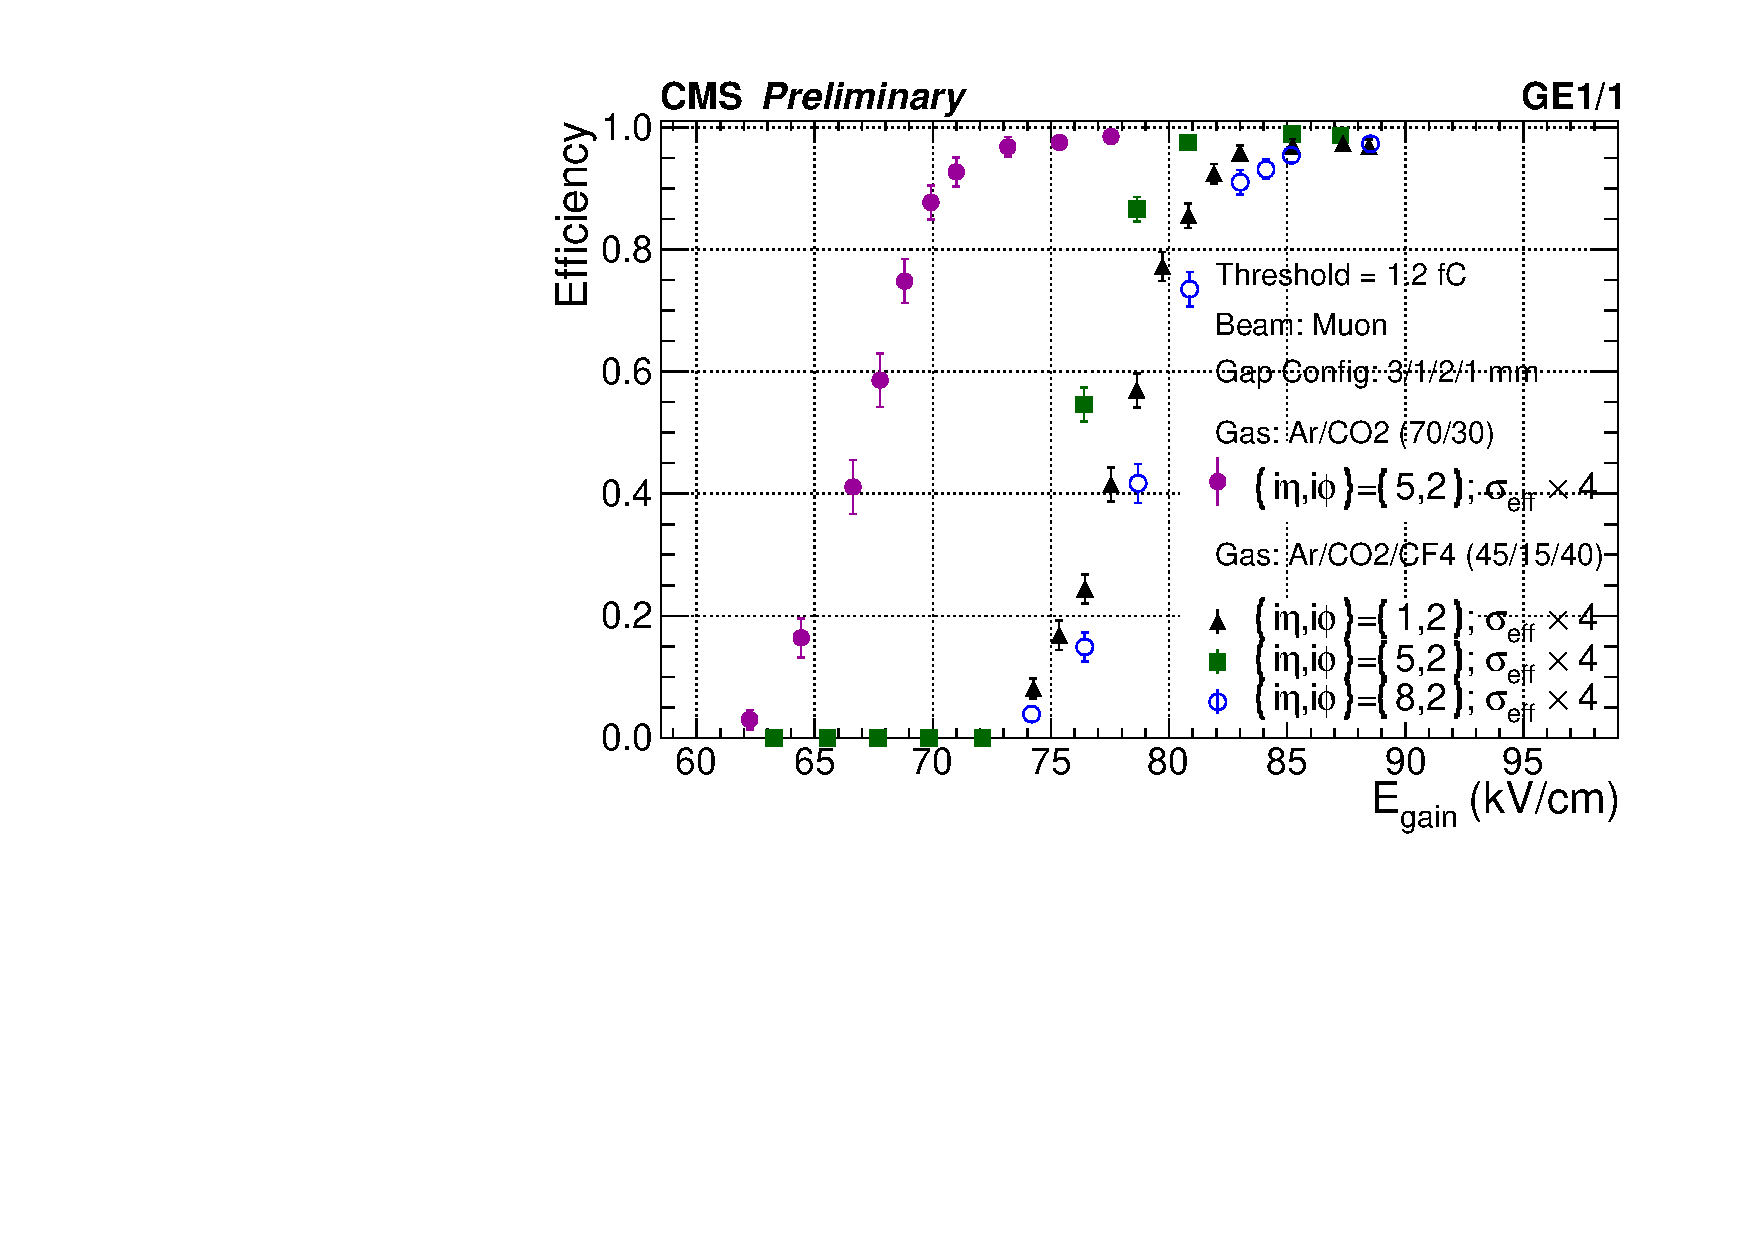
\includegraphics[width=3.5in]{figures/GEM/EfficiencyPlot_wrt_EGain_wError4times_2gas.pdf}
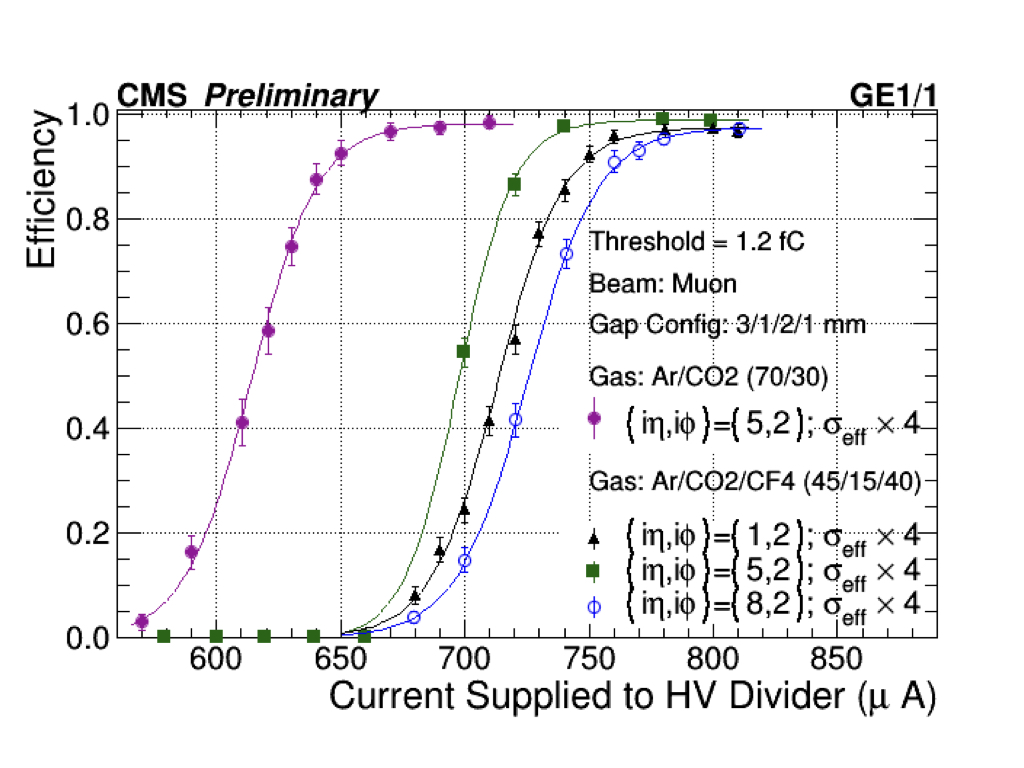
\includegraphics[width=0.75\textwidth]{figures/GEM/Efficiency_Current.jpeg}
\caption{Efficiency w.r.t. current supplied to high voltage divider for two different gases and three different $(i\eta,i\phi)$ sectors.}
\label{Efficiency}
\end{figure}
Here, the efficiency is fitted with function:
\begin{equation}\label{EfffitEq}
    Efficiency = \frac{Eff_{max}}{1+e^{s(HV-HV_{50\%})}}
\end{equation}
Where, $Eff_{max}$ is the maximum obtained efficiency, $HV_{50\%}$ is the applied HV (or current or $E_{gain}$) when corresponding efficiency becomes 50\% and $s$ is just a scale factor.

\subsection{Fit Parameters} % (fold)
\label{sub:fit_parameters}
Lets define four different function, based on equation~\ref{EfffitEq}, F1 for $(i\eta,i\phi)$ sector (5,2) with gas $Ar/CO_2/CF_4$, F2 for $(i\eta,i\phi)$ sector (1,2) with gas $Ar/CO_2/CF_4$, F3 for $(i\eta,i\phi)$ sector (8,2) with gas $Ar/CO_2/CF_4$ and F4 for $(i\eta,i\phi)$ sector (5,2) with gas $Ar/CO_2$.
% subsection fit_parameters (end)

After fit F1 is given as
\begin{equation}
	F1 = [0] + \frac{0.989}{[1]+exp(-[2]\times(x-697.3))}
\end{equation}
where,
% $[0] = -1.44526e-02 \pm 4.28771e-02$, \\$[1] = 9.84833e-01 \pm 4.19715e-02$ and \\$[2] = 9.97591e-01 \pm 8.53940e-02$
\begin{align*}
[0] &= -1.44526e-02 \pm 4.28771e-02,\\
[1] &= 9.84833e-01 \pm 4.19715e-02,~and \\
[2] &= 9.97591e-01 \pm 8.53940e-02
\end{align*}

After fit F2 is given as
\begin{equation}
	F2 = \frac{0.968}{[0]+exp(-[1]\times(x-64.9))}
\end{equation}
where,
\begin{align*}
[0] &= 9.92180e-01 \pm 5.56034e-03,\\
[1] &= 8.25180e-01 \pm 3.62098e-02
\end{align*} 

After fit F3 is given as
\begin{equation}
	F3 = \frac{0.973}{[0]+exp(-[1]\times(x-66))}
\end{equation}
where,
\begin{align*}
[0] &= 9.96407e-01 \pm 9.00503e-03, \\
[1] &= 7.67029e-01 \pm 4.59276e-02
\end{align*}


After fit F4 is given as
\begin{equation}
	F4 = \frac{0.985}{[0]+exp(-[1]\times(x-55.8))}
\end{equation}
where,
\begin{align*}
[0] &= 1.00305e+00 \pm 7.91473e-03,\\
[1] &= 8.15287e-01 \pm 5.46309e-02
\end{align*}



% section efficiency_vs_ (end)


\section{Efficiency Vs Drift Voltage} % (fold)
\label{sec:efficiency_vs_Drift_Voltage}
\begin{figure}[!htbp]
\centering
% 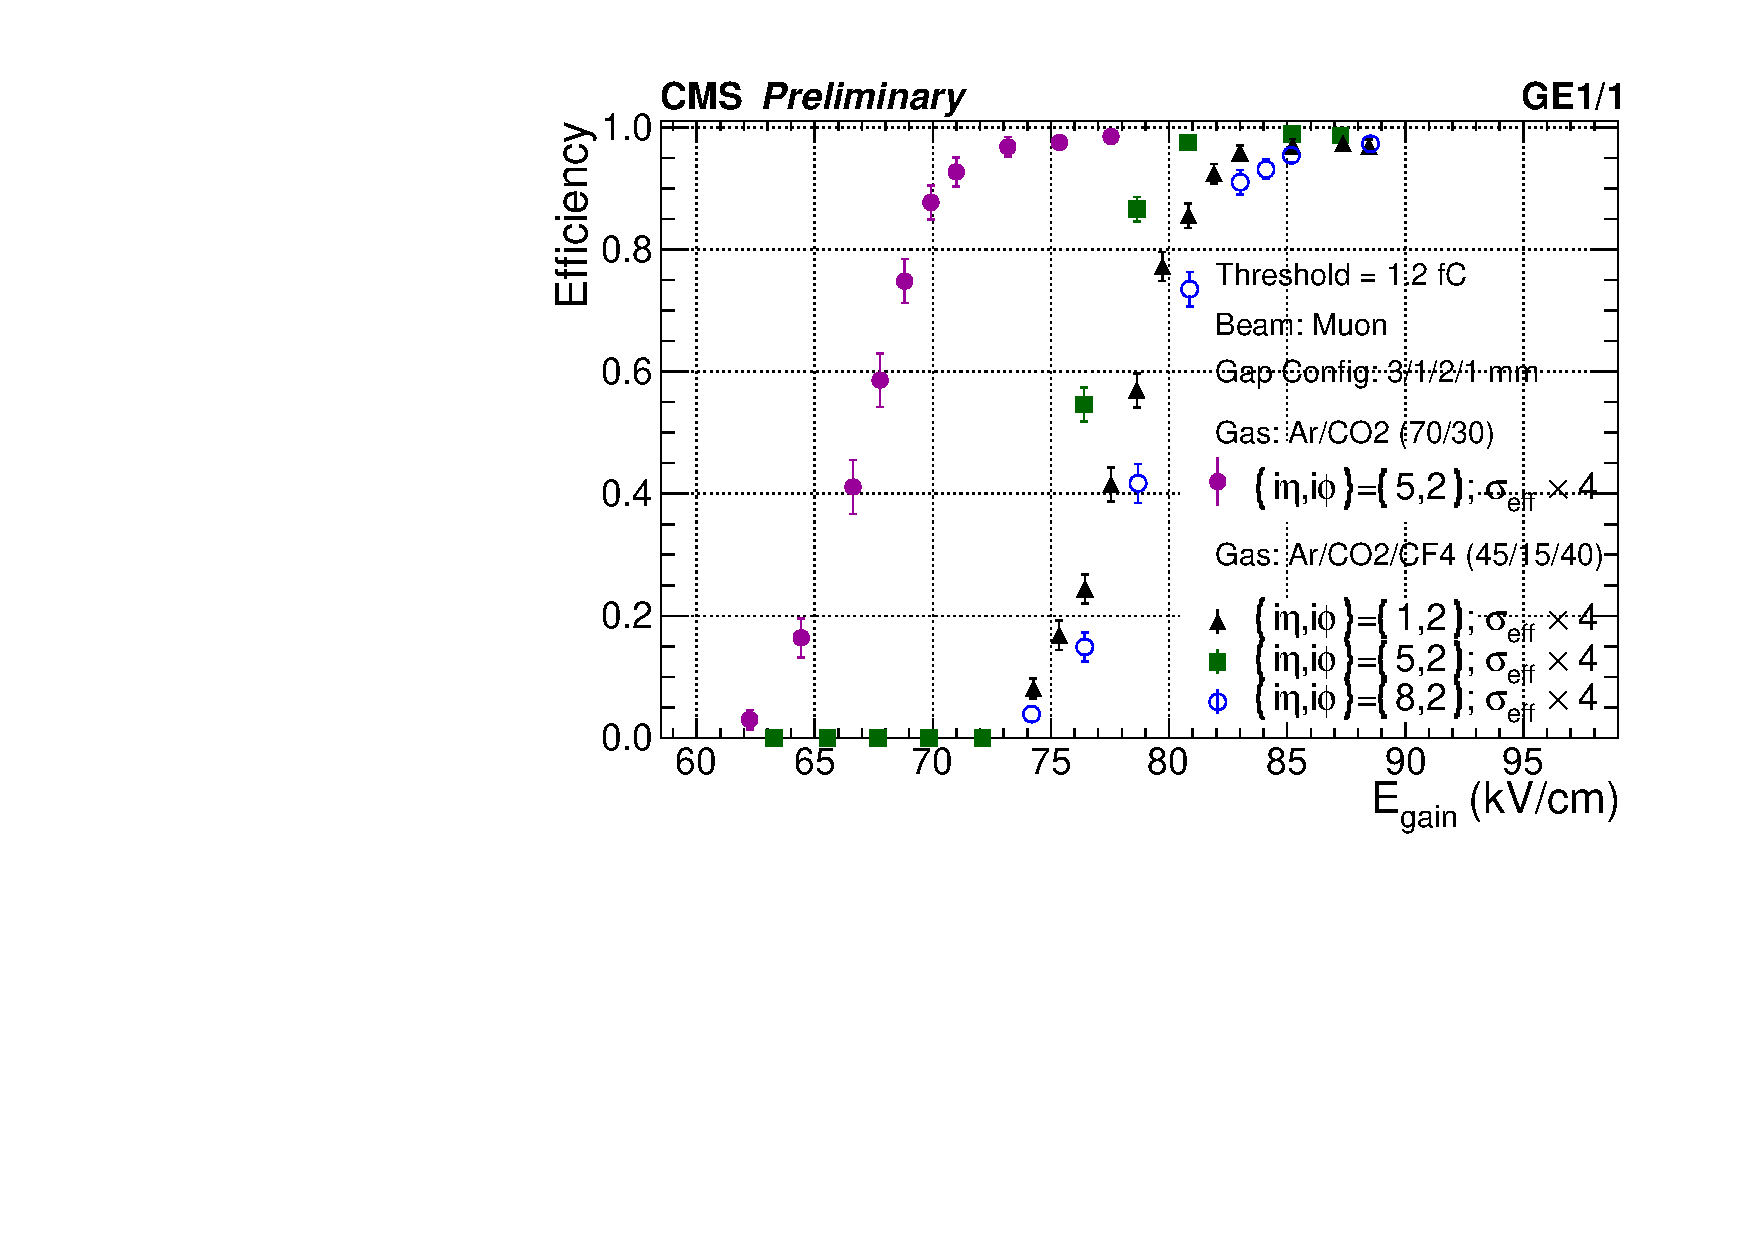
\includegraphics[width=3.5in]{figures/GEM/EfficiencyPlot_wrt_EGain_wError4times_2gas.pdf}
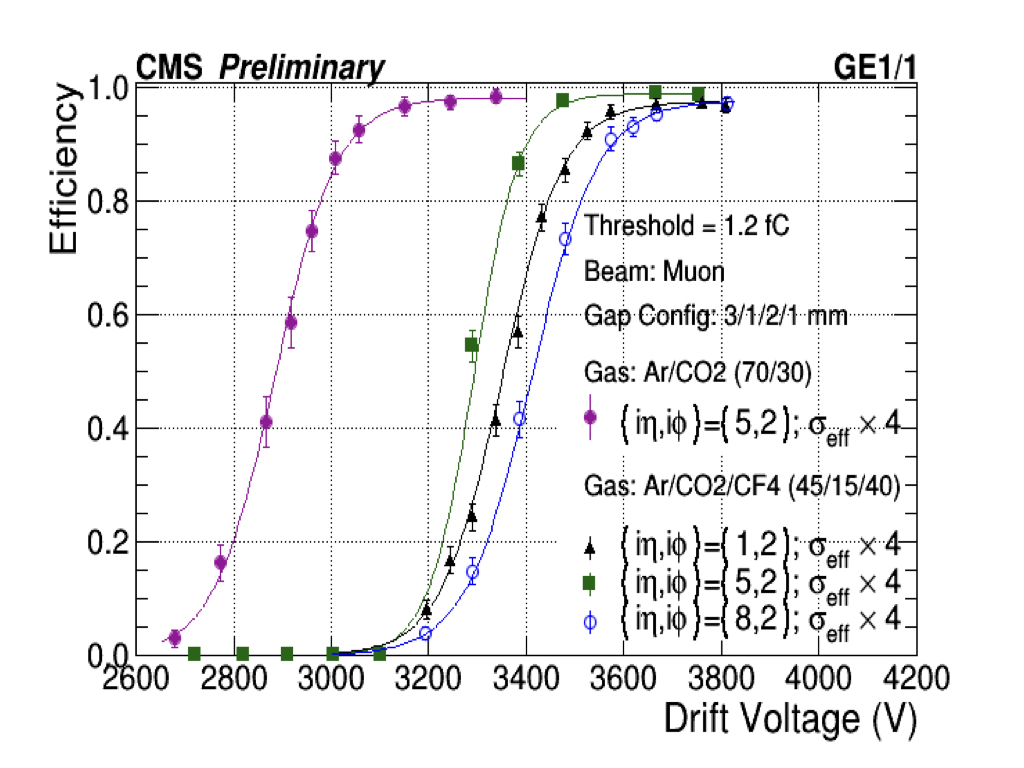
\includegraphics[width=0.75\textwidth]{figures/GEM/Efficiency_DriftVoltage.jpeg}
\caption{Efficiency w.r.t. drift voltage for two different gases and three different $(i\eta,i\phi)$ sectors.}
\label{Efficiency}
\end{figure}
Here, the efficiency is fitted with function:
\begin{equation}\label{EfffitEq}
    Efficiency = \frac{Eff_{max}}{1+e^{s(HV-HV_{50\%})}}
\end{equation}
Where, $Eff_{max}$ is the maximum obtained efficiency, $HV_{50\%}$ is the applied HV (or current or $E_{gain}$) when corresponding efficiency becomes 50\% and $s$ is just a scale factor.

\subsection{Fit Parameters} % (fold)
\label{sub:fit_parameters}
Lets define four different function, based on equation~\ref{EfffitEq}, F1 for $(i\eta,i\phi)$ sector (5,2) with gas $Ar/CO_2/CF_4$, F2 for $(i\eta,i\phi)$ sector (1,2) with gas $Ar/CO_2/CF_4$, F3 for $(i\eta,i\phi)$ sector (8,2) with gas $Ar/CO_2/CF_4$ and F4 for $(i\eta,i\phi)$ sector (5,2) with gas $Ar/CO_2$.
% subsection fit_parameters (end)

After fit F1 is given as
\begin{equation}
	F1 = [0] + \frac{0.989}{[1]+exp(-[2]\times(x-697.3))}
\end{equation}
where,
% $[0] = -1.44526e-02 \pm 4.28771e-02$, \\$[1] = 9.84833e-01 \pm 4.19715e-02$ and \\$[2] = 9.97591e-01 \pm 8.53940e-02$
\begin{align*}
[0] &= -1.44526e-02 \pm 4.28771e-02,\\
[1] &= 9.84833e-01 \pm 4.19715e-02,~and \\
[2] &= 9.97591e-01 \pm 8.53940e-02
\end{align*}

After fit F2 is given as
\begin{equation}
	F2 = \frac{0.968}{[0]+exp(-[1]\times(x-64.9))}
\end{equation}
where,
\begin{align*}
[0] &= 9.92180e-01 \pm 5.56034e-03,\\
[1] &= 8.25180e-01 \pm 3.62098e-02
\end{align*} 

After fit F3 is given as
\begin{equation}
	F3 = \frac{0.973}{[0]+exp(-[1]\times(x-66))}
\end{equation}
where,
\begin{align*}
[0] &= 9.96407e-01 \pm 9.00503e-03, \\
[1] &= 7.67029e-01 \pm 4.59276e-02
\end{align*}


After fit F4 is given as
\begin{equation}
	F4 = \frac{0.985}{[0]+exp(-[1]\times(x-55.8))}
\end{equation}
where,
\begin{align*}
[0] &= 1.00305e+00 \pm 7.91473e-03,\\
[1] &= 8.15287e-01 \pm 5.46309e-02
\end{align*}
% chapter efficiency_and_time_resolution_fit_parameters (end)